
\section{ĐẠI SỐ}
\setcounter{ex}{0}
%1
\begin{ex}
	Trong các tập hợp sau, tập hợp nào có các phần tử đều là số nguyên tố? 
	\choice
	{$\{1;3;5;7;19\}$}
	{$\{2;3;5;7;9\}$}
	{\True $\{2;3;5;7;11\}$}
	{$\{0;3;5;7;13\}$}		
\end{ex}
%2
\begin{ex} Tập hợp $A = \{0; 1; 2; 3; 4; 5; 6; 7; 8; 9; 10\}$. Phát biểu nào sau đây là đúng?
	\choice
	{$11 \in A$}
	{$1 \notin A$}
	{\True $10 \in A$}
	{$7 \notin A$}
\end{ex}
%3
\begin{ex}
	Trong một hội nghị có 100 đại biểu tham dự. Mỗi đại biểu nói được một hoặc hai hoặc ba \\
	\begin{minipage}{0.6\textwidth}
	 thứ tiếng: Nga, Anh hoặc Pháp. Biết rằng có 39 đại biểu chỉ nói được tiếng Anh, 35 đại biểu nói được tiếng Pháp, 8 đại biểu nói được cả tiếng Anh và tiếng Nga. Hỏi có bao nhiêu đại biểu chỉ nói được tiếng Nga?
	
	
		\hfill
		\choice
		{$26$ đại biểu}
		{$53$ đại biểu}
		{\True $18$ đại biểu}
		{$20$ đại biểu}
	\end{minipage}
	\begin{minipage}{0.4\textwidth}
		
			%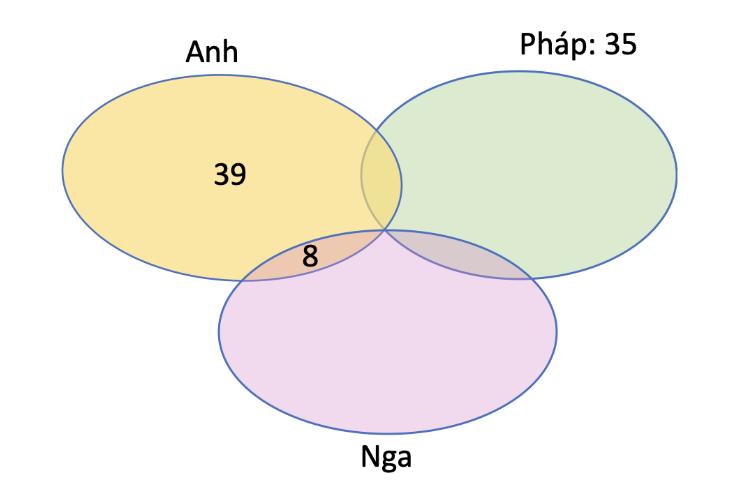
\includegraphics[scale=0.3]{data/Hình/H2}\\
		
		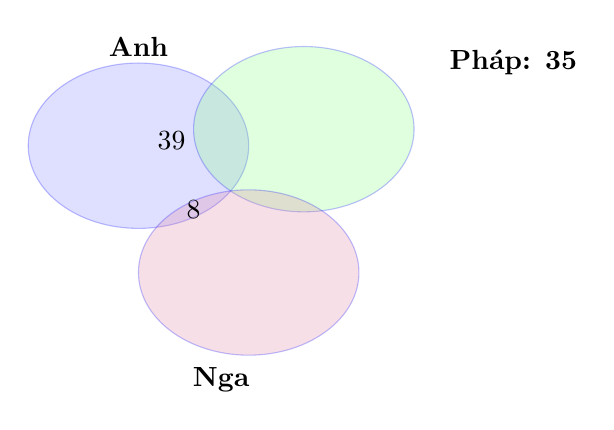
\begin{tikzpicture}[scale=0.7]
			
			%--- Ellipse Anh ---
			\fill[blue!50, opacity=0.25, draw=blue]
			(-1.5,0) ellipse (2 and 1.5);
			
			%--- Ellipse Pháp ---
			\fill[green!50, opacity=0.25, draw=blue]
			(1.5,0.3) ellipse (2 and 1.5);
			
			%--- Ellipse Nga ---
			\fill[purple!50, opacity=0.25, draw=blue]
			(0.5,-2.3) ellipse (2 and 1.5);
			
			%--- Labels ---
			\node at (-1.5,1.8) {\bf Anh};
			\node at (5.3,1.5) {\bf Pháp: 35};
			\node at (0,-4.25) {\bf Nga};
			
			%--- Numbers ---
			\node at (-0.9,0.1) {39};
			\node at (-0.5,-1.15) {8};
			
		\end{tikzpicture}
		
	\end{minipage}%
\end{ex}
%4
	\begin{ex} % Câu 1%[6D1B5-6]%[Dự án đề kiểm tra Toán 6 HKI NH23-24-NGUYỄN VĂN HỮU]%[THCS TÂN TRÀO]
	Kết quả phép tính $3^{2023}$ $:$ $3^{2020}$ là
	\choice
	{$3^{4}$}
	{$27$}
	{$3^{3}$}
	{\True Cả B, C đều đúng}
\end{ex}
%5
\begin{ex}%[6D1Y8-1]%[Dự án đề kiểm tra Toán 7 HKI NH23-24- Nguyễn Văn Hiệp]%[THCS Qui Đức]
	Số nào sau đây chia hết cho cả $2$, $3$	và $5$ nhưng không chia hết cho $9$?
	\choice
	{\True $240$}
	{$270$}
	{$235$}
	{$532$}
\end{ex}
%6
\begin{ex}%%câu 1
	Khẳng định nào sau đây \textbf{sai}?
	\choice
	{Nếu $a\ \vdots\ 3$ và $b\ \vdots\ 3$ thì $(a+b)\ \vdots\ 3$}
	{Nếu $a\ \vdots\ 2$ và $b\ \vdots\ 2$ thì $(a-b)\ \vdots\ 2$}
	{Nếu $a\ \vdots\ 4$ và $b\not\vdots\ 4$ thì $(a+b)\not\vdots\ 4$}
	{\True Nếu $a\ \vdots\ 5$ và $b\ \vdots\ 4$ thì $(a+b)\ \vdots\ 20$}	
\end{ex}
%7
\begin{ex} Hợp số là gì: 
	\choice
	{Hợp số là số tự nhiên}
	{Hợp số là số tự nhiên khác 0 có hai ước}
	{Hợp số là số tự nhiên khác 0 có nhiều hơn hai ước}
	{\True Hợp số là số tự nhiên lớn hơn 1 và có nhiều hơn hai ước}
\end{ex}

\begin{ex}%[6D1BC-2]%[Dự án đề kiểm tra HKI NH23-24- Dương BùiĐức]
	ƯCLN($12; 36$) bằng
	\choice
	{$15$}
	{$30$}
	{$6$}
	{\True $12$}
\end{ex}

\begin{ex}%[6D1KD-3] %[Dự án đề kiểm tra Toán 6 HKI NH23-24-NGUYỄN VĂN HỮU]%[THCS TÂN TRÀO]
	Tìm tất cả Bội chung nhỏ hơn $ 100 $ của $ 7 $ và $ 6 $ ?
	\choice
	{\True $\{0 ; 42 ; 84\}$}
	{$\{42 ; 84\}$}
	{$\{84\}$}
	{$\{42\}$}
\end{ex}


\begin{ex}%[6D1KC-3] %[Dự án đề kiểm tra Toán 6 HKI NH23-24- Phạm Văn Long]%[THCS Bình Chánh]
	Lớp 6A có $21$ bạn nam và $27$ bạn nữ. Trong tiết Toán, thầy Lâm yêu cầu lớp trưởng tiến hành chia nhóm để các bạn hoạt động xây dựng bài học mới, sao cho số bạn nam và nữ trong mỗi nhóm bằng nhau. Số nhóm nhiều nhất trong lớp có thể chia được là:
	\choice
	{\True $3$}
	{$4$}
	{$5$}
	{$6$}
\end{ex}

\begin{ex} %[6D1TD-3]
	Bốn chiếc đồng hồ reo chuông tương ứng sau mỗi $5$ phút, $10$ phút, $15$ phút và $20$ phút. Chúng bắt đầu cùng reo chuông vào lúc $12$ giờ trưa. Lần tiếp theo chúng cùng reo chuông vào lúc nào?
	\choice
	{\True $13$ giờ trưa}
	{$13$ giờ $20$ trưa}
	{$12$ giờ $45$ trưa}
	{$12$ giờ $30$ trưa}
\end{ex}

\begin{ex}%[6D1KB-2]
	Một lớp có $42$ học sinh. Hỏi có bao nhiêu cách chia tổ, biết rằng số học sinh sau khi chia vào các tổ phải bằng nhau và số tổ lớn hơn $3$, nhỏ hơn $7$?
	\choice
	{\True Có $1$ cách chia tổ} 	
	{Có $6$ cách chia tổ}
	{Có $3$ cách chia tổ}	
	{Có $8$ cách chia tổ}
\end{ex}

\begin{ex}
	Số nào sau đây là số nguyên?
	\choice
	{$-0{,}8$}
	{\True $-8$}
	{$3{,}2$}
	{$\dfrac{-5}{2}$}
\end{ex}

\begin{ex} %C11
	Trong các tập hợp sau, tập hợp nào có các phần tử được xếp theo thứ tự tăng dần:
	\choice
	{$\{2;-17;5;1;-2;0\}$}
	{$\{-2;-17;0;1;2;5\}$}
	{\True $\{-17;-2;0;1;2;5\}$}
	{$\{0;1;2;5;-17\}$}
\end{ex}

\begin{ex}%[6D2B2-2]
	Các vị trí $a$, $b$, $c$ ở hình sau đây biểu diễn các số nguyên nào?
	\begin{center}
		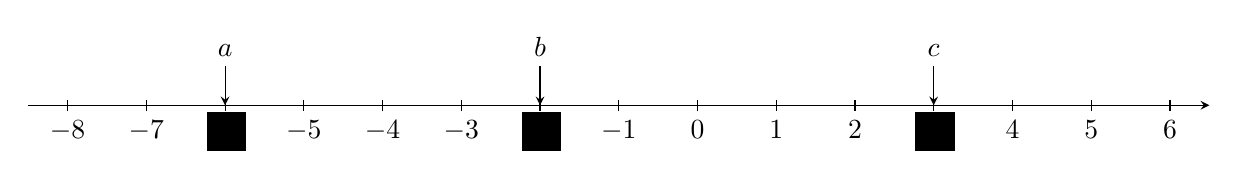
\begin{tikzpicture}[>=stealth]
			\draw[->] (-8.5,0)--(6.5,0);
			\foreach \x in {-8,...,6}
			\draw[shift={(\x,0)}] (0,2pt)--(0,-2pt) node[below]{ $\x$};
			\foreach \x/\y in {-6/a,-2/b,3/c}{
				\draw[<-] (\x,0)--++(90:.5)node[above]{$\y$};
				\fill ([shift={(200:.25)}]\x,0) rectangle ++(.5,-.5);
			}
			
		\end{tikzpicture}
	\end{center}
	\choice
	{\True $-6$; $-2$ và $3$}
	{$3$; $-2$ và $-6$}
	{$2$ và $6$}
	{$-2$ và $-6$}
	
\end{ex}

\begin{ex}%C8
	Số đối của $-(-a)$ là
	\choice
	{\True $-a$}
	{$a$}
	{$0$}
	{$1$}
\end{ex}

\begin{ex}%[6D2B4-1]%[Dự án đề kiểm tra HKI NH23-24- Dương BùiĐức]
	Kết quả phép tính $-268+47-32+53$ là
	\choice
	{\True $- 200$}
	{$200$}
	{$336$}
	{$-336$}
\end{ex}

\begin{ex}  %[6D1Y4-1]
	Kết quả của phép tính $(50-20):(-2)+1$ là
	\choice
	{\True $-14$}
	{$14$}
	{$16$}
	{$-16$}
\end{ex}

\begin{ex}%C9
	Nhận định nào sau đây đúng?
	\choice
	{$(-4) \cdot 8>0$}
	{$(-4) .(-8)<0$}
	{\True $4 .(-8)<0$}
	{$(-4) \cdot(-8)=-32$}
\end{ex}


\begin{ex}
	Tính tổng tất cả số nguyên $x$ thỏa $-3<x<3$ là
	\choice
	{$-3$}
	{$3$}
	{$6$}
	{\True $0$}
\end{ex}

\begin{ex} Tìm số nguyên $x$, thỏa mãn: $x^2=81$
	\choice
	{$x=9$}
	{$x=-9$}
	{\True $x=9$ hoặc $x=-9$}
	{$x=3$}
\end{ex}	
%22
\begin{ex}
	Tập hợp các ước nguyên của $9$ là	
	\choice
	{Ư$(9) = \{0; 1; -1; 3; -3; 9; -9\}$}
	{Ư$(9) = \{ 1; -1; 3; -3; 6; 9\}$}
	{\True Ư$(9) = \{ 1; -1; 3; -3; 9; -9\}$}
	{Ư$(9) = \{1; 3; 6; 9\}$}	
\end{ex}

\begin{ex}
	Lợi nhuận của công ty An Bình trong $4$ tháng đầu năm là $-40$ triệu đồng mỗi tháng. Lợi nhuận trong $8$ tháng sau đó là $80$ triệu mỗi tháng. Hỏi sau $1$ năm công ty An Bình có lợi nhuận là bao nhiêu triệu đồng?
	\choice
	{$120$} 
	{\True $480$}
	{$40$} 
	{$420$}
\end{ex}

%Câu 3
\begin{ex}
	Một tàu ngầm đang ở độ sâu $20$ m, nếu tàu ngầm tiếp tục lặn xuống thêm $15$ m nữa, khi đó tàu ngầm ở độ cao so với mực nước biển là
	\choice
	{\True $-35$ m}
	{$-5$ m}
	{$15$ m}
	{$35$ m}
\end{ex}

%%%============CÂU 25 ==============%%%

\begin{ex} %[6D2T4-1]
	Ban ngày, nhiệt độ ở New York (Niu Oóc) là $-5^{\circ} {C}$. Nhiệt độ ban đêm là $-14^{\circ} {C}$. Tính chênh lệch nhiệt độ giữa ngày và đêm ở New York?
	\choice
	{$-19^{\circ} {C}$}
	{$-9^{\circ} {C}$}
	{\True $9^{\circ} {C}$}
	{$19^{\circ} {C}$}
\end{ex}




